\begin{figure}[H]
	\centering
	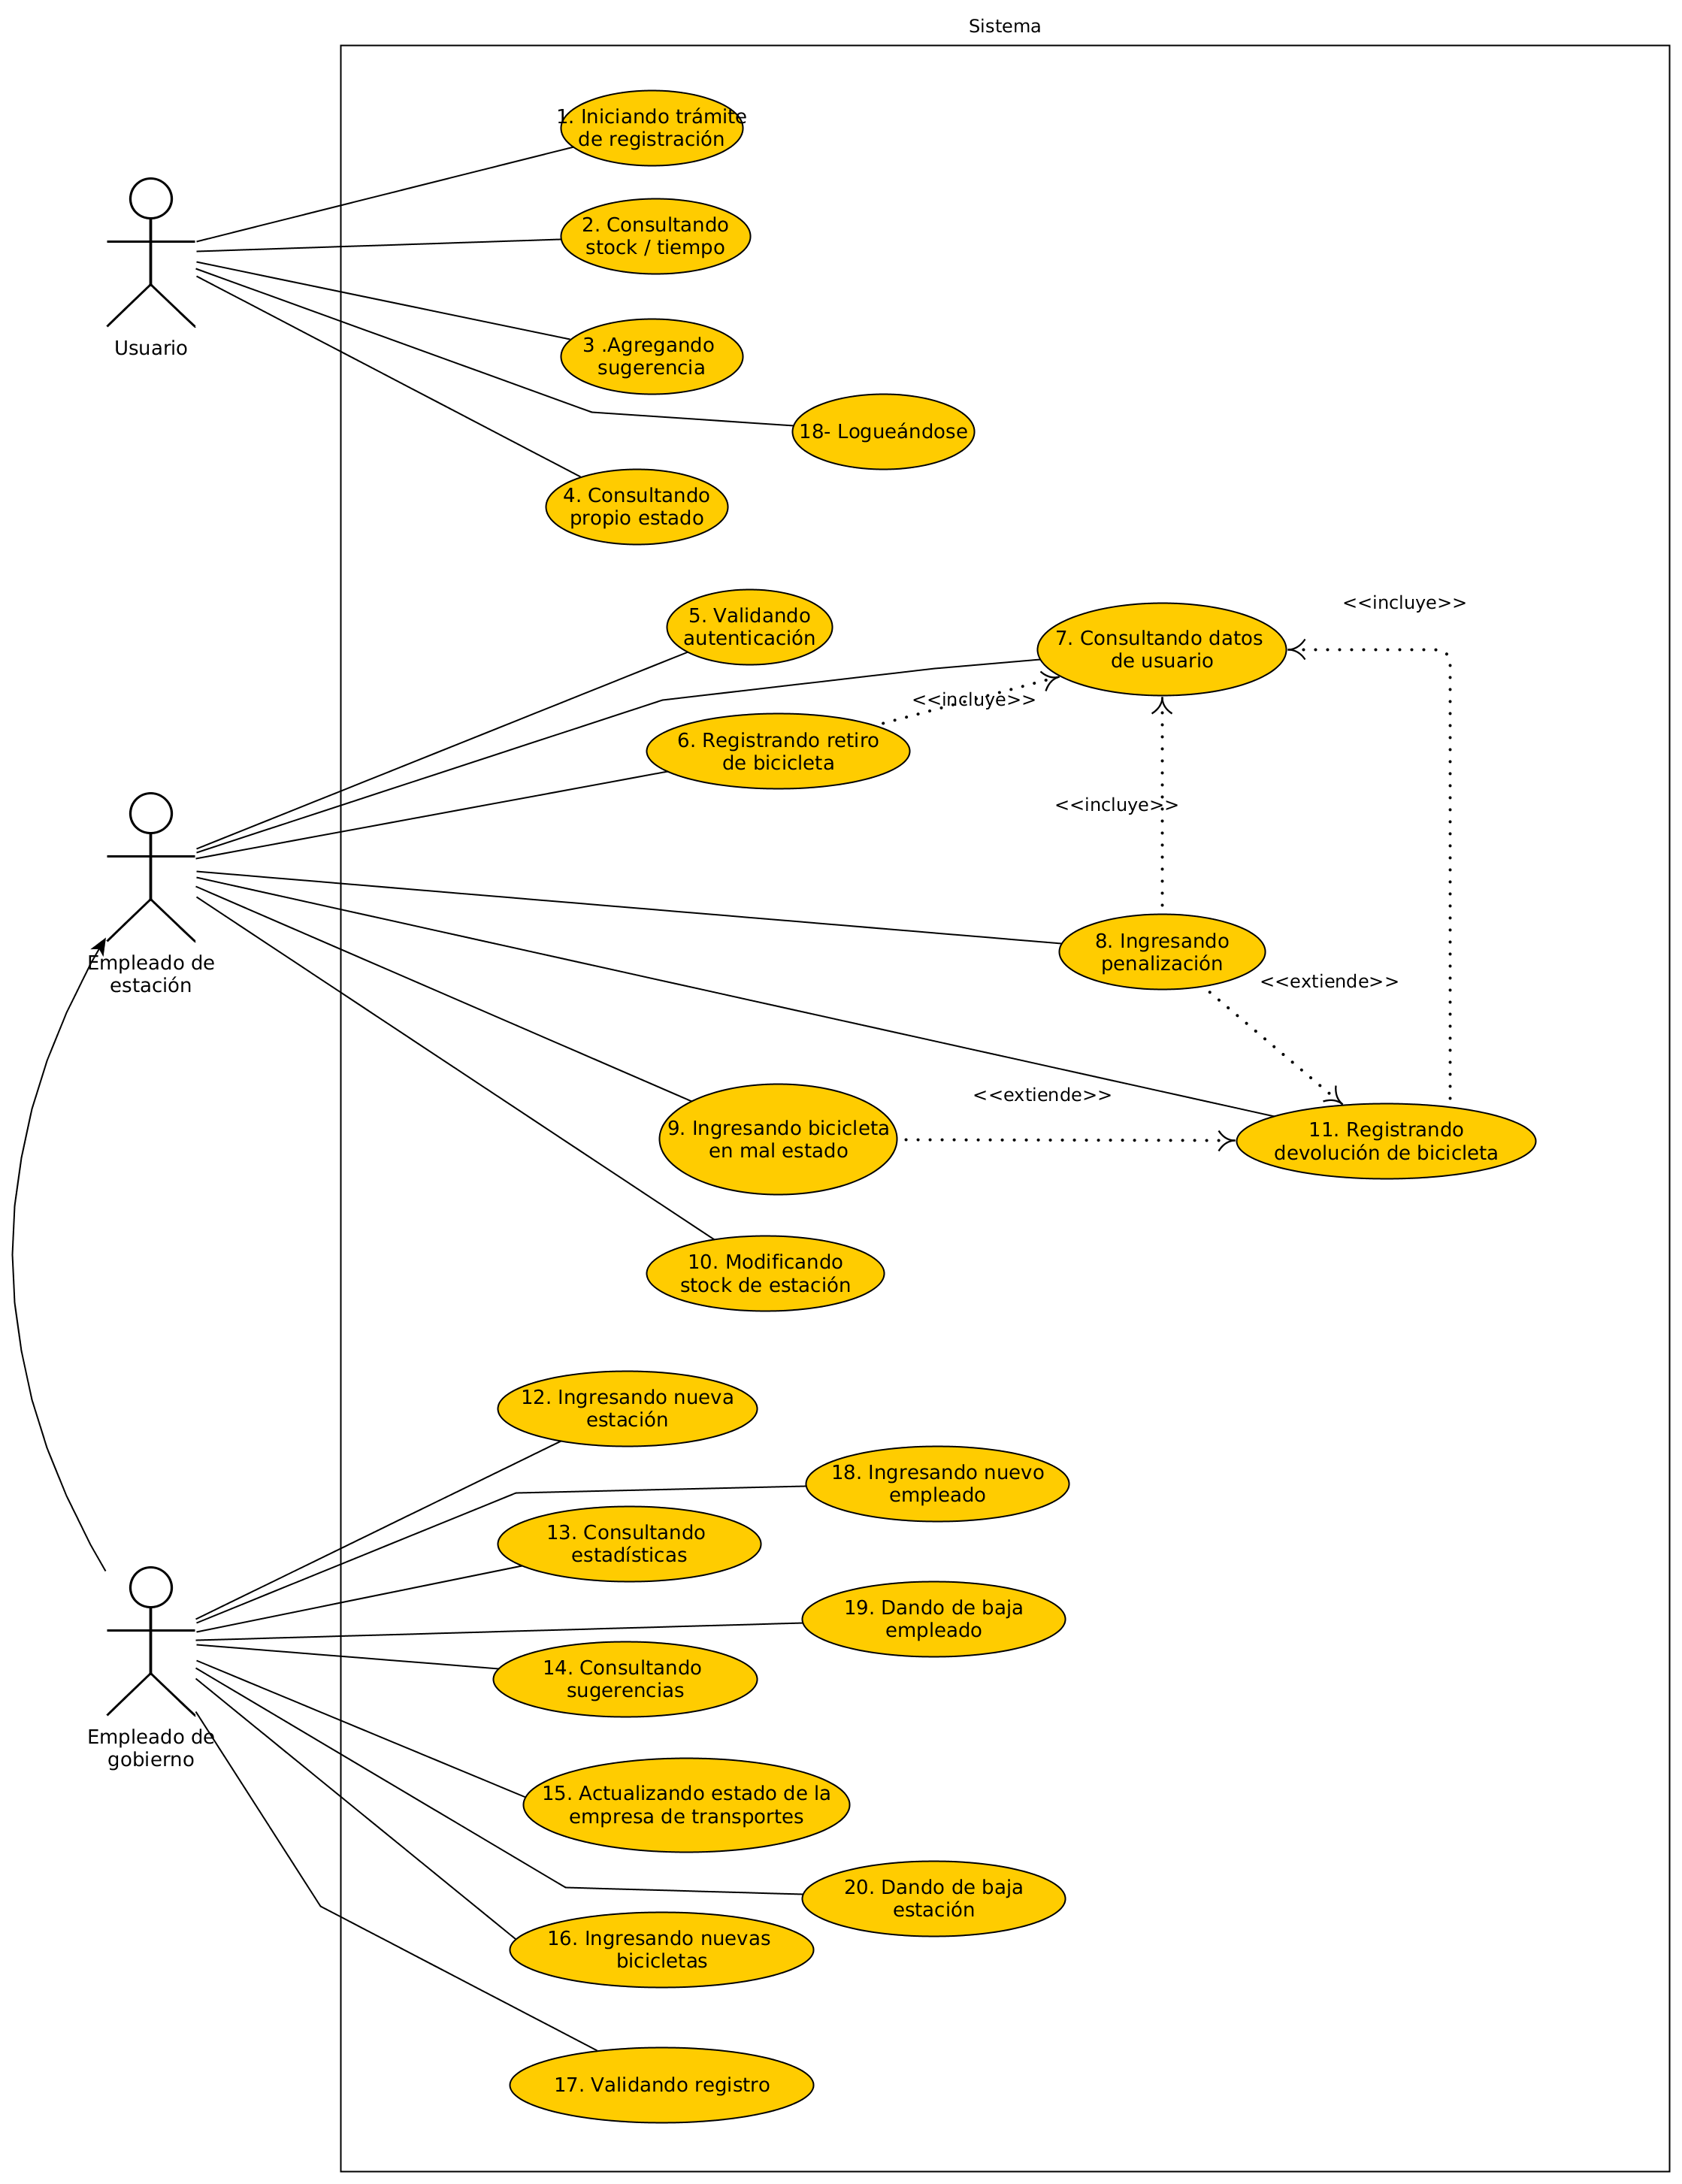
\includegraphics[scale=0.2]{imgs/casos_de_uso.png}
	\caption{Casos de uso}
\end{figure}

\subsection{Usuario}

~

\cu{Iniciando trámite de registración}{Usuario}{}{1}

\begin{center}
    \centering
    \begin{tabular}{ | p{11cm} | p{6cm} | }
    	\multicolumn{1}{c}{\cellcolor{black!30}\textbf{Curso normal}} & 
    	\multicolumn{1}{c}{\cellcolor{black!30}\textbf{Curso alternativo}} \\
		\hline
		1- El sistema despliega una interfaz gráfica con campos a completar
		por el usuario: Nombre completo, Número de DNI, Domicilio, Mail, teléfono
		de contacto y una contrase\~na para poder loguearse & \\ \hline
		2 - El usuario ingresa los datos en el sistema & 2.1 - El usuario ya se encuentra ingresado en el sistema
		o hay una inconsistencia con los datos de otro usuario almacenado en la base de datos. Fin de C.U \\ \hline
		3 - El sistema registra al usuario en el sistema, almacena los datos en la base de datos y le anuncia al usuario que la registración se completará cuando los datos se validen y que se le comunicará de dicha operación via email.& \\ \hline
		\underline{Postcondición :} Trámite de registración iniciado & \\ \hline
    \end{tabular}
\end{center}

Una vez que el registro es realizado, los datos quedan sujetos a verificación por parte de un empleado de gobierno.

~

\cu{Logueándose}{Usuario}{}{18}
\begin{center}
    \centering
    \begin{tabular}{ | p{11cm} | p{6cm} | }
    	\multicolumn{1}{c}{\cellcolor{black!30}\textbf{Curso normal}} & 
    	\multicolumn{1}{c}{\cellcolor{black!30}\textbf{Curso alternativo}} \\
		\hline
		1- El sistema solicita al usuario que ingrese su número de DNI y su contrase\~na para poder loguearse
		&  \\ \hline
		2 - El usuario ingresa los datos requeridos & 2.1 - El sistema detecta una inconsistencia en los datos ingresados y
		solicita que los ingrese nuevamente \\ \hline
		3 - El sistema le informa al usuario que se ha logueado exitosamente & \\ \hline
		\underline{Postcondición :} Usuario logueándose & \\ \hline
    \end{tabular}
\end{center}

Para que un usuario pueda loguearse es necesario que esté registrado. Sin embargo, esto no puede ser una precondición ya que
eventualmente cualquier persona puede realizar el intento de loguearse. La contrase\~na que el usuario debe ingresar debe
corresponderse con aquella elegida al momento de iniciar el trámite de registración.

~

\cu{Consultando stock/tiempo}{Usuario}{Trámite de registración iniciado}{2}
\begin{center}
    \centering
    \begin{tabular}{ | p{11cm} | p{6cm} | }
    	\multicolumn{1}{c}{\cellcolor{black!30}\textbf{Curso normal}} & 
    	\multicolumn{1}{c}{\cellcolor{black!30}\textbf{Curso alternativo}} \\
		\hline
		1- El usuario le informa al sistema que desea realizar una consulta acerca de la disponibilidad
		de bicicletas en una determinada estación & \\ \hline
		2- El sistema despliega una lista con las estaciones que es posible consultar & 
		2.1- El usuario no encuentra en la lista la estación que está buscando porque la misma no se encuentra en
		funcionamiento, con lo cual o bien procede a consultar disponibilidad en una estación cercana (ir al paso 3), o
		decide finalizar la consulta (Fin de C.U)\\ \hline
		3- El usuario selecciona la estación sobre la cual desea consultar. & \\ \hline
		4- El sistema envía información acerca de la disponibilidad en la estación seleccionada al momento de la consulta, utilizando distintos colores para reforzar el contenido del mensaje. En el caso de haber muchas bicicletas disponibles utiliza el color verde. Si hay una cantidad moderada de bicicletas utiliza el color naranja. Finalmente,
		si la cantidad de bicicletas disponibles está por agotarse utiliza el color rojo. Si por el contrario no hay
		bicicletas disponibles en la estación el sistema informa este hecho al usuario y envía un tiempo estimado en el cual
		es probable que el stock vuelva a ser positivo. & \\ \hline
		\underline{Postcondición :} Consulta realizada & \\ \hline
    \end{tabular}
\end{center}	

Para este caso de uso no es necesario que el usuario haya iniciado el trámite de registración ya que según los
requerimientos cualquiera puede obtener esta información.

~

\cu{Consultando propio estado}{Usuario}{Usuario logueado}{3}
\begin{center}
    \centering
    \begin{tabular}{ | p{11cm} | p{6cm} | }
    	\multicolumn{1}{c}{\cellcolor{black!30}\textbf{Curso normal}} & 
    	\multicolumn{1}{c}{\cellcolor{black!30}\textbf{Curso alternativo}} \\
		\hline
		1- El usuario le informa al sistema que desea consultar su estado & \\ \hline
		2- El sistema le despliega una interfaz con varias opciones a consultar:
		existencia de penalización actual, el historial de 
		penalizaciones y el historial de alquileres. & \\ \hline
		3- El usuario indica la opción que desea consultar & \\ \hline
		4- El sistema le envía al usuario la información solicitada.
		\underline{Postcondición :} Consulta individual realizada & \\ \hline
    \end{tabular}
\end{center}

Para este caso de uso es una precondición que el usuario esté logueado, ya que la información consultada es confidencial, por
lo que es consistente respecto a los requerimientos de seguridad planteados en el diagrama de objetivos durante la primera 
iteración (Evitar suplantación de identidad)

~

\cu{Agregando sugerencia}{Usuario}{Usuario logueado}{4}
\begin{center}
    \centering
    \begin{tabular}{ | p{11cm} | p{6cm} | }
    	\multicolumn{1}{c}{\cellcolor{black!30}\textbf{Curso normal}} & 
    	\multicolumn{1}{c}{\cellcolor{black!30}\textbf{Curso alternativo}} \\
		\hline
		1- El usuario le informa al sistema que desea enviar una sugerencia & \\ \hline
		2- El sistema despliega un cuadro de texto en donde el usuario puede escribir los comentarios,
		mostrando también las pautas del correcto uso de dicha herramienta (Solicita
		utilizar el espacio con
		responsabilidad evitando el uso indebido del lenguaje).
		También muestra ejemplos de comentarios que han ayudado a la mejora de las ciclovías. & \\ \hline
		3- El usuario ingresa sus comentarios y los envía al sistema & \\ \hline
		4- El sistema le indica al usuario que las sugerencias han sido almacenadas & \\ \hline
		\underline{Postcondición :} Sugerencia enviada & \\ \hline
    \end{tabular}
\end{center}




